\documentclass[15pt,t]{beamer}
\usepackage{xcolor}
\usepackage{IEEEtrantools}
\usepackage{pgf}  % PGF/TikZ is needed for nice plots
\usepackage[cmex10]{mathtools} % for math equations
\usepackage{csquotes}
\usepackage{amsthm}
\usepackage{scalefnt}
\usepackage[utf8]{inputenc}
\usepackage[T1]{fontenc}
\usepackage{lipsum, lmodern}
\usepackage{amsmath,amsfonts,amsthm, latexsym,mathtools,mathrsfs}
\usepackage{geometry}
\geometry{textwidth=7cm}
\usepackage{amssymb}
\usepackage{graphicx}
%\usepackage{epstopdf}
\usepackage{rotating}
\usepackage{multirow}
\usepackage{filecontents}
\usepackage{ragged2e}
\usepackage{subfig}
\usepackage{varwidth}
\usepackage{bm}
\usepackage{lipsum}
\setlength\parindent{0pt}

\addtobeamertemplate{block begin}{}{\justifying}  %new code


\graphicspath{{./graphics/}}

\usetheme{purduegold}

%\usepackage{enumitem}
\setbeamersize{text margin left=3mm,text margin right=3mm} 
%\addtobeamertemplate{frametitle}{}{\vspace{1em}} % increase
%\addtobeamertemplate{frametitle}{}{\vspace*{-15mm}} % decrease

%\setstretch{1.25}
\usepackage{enumitem}
\usepackage{uarial}
\usebeamercolor*{normal text}
\usefonttheme[stillsansseriflarge]{serif}
\definecolor{azure}{rgb}{0.0, 0.5, 1.0}



\author{Bhisham (D18039) \& Himanshu (V18011)}
\beamerdefaultoverlayspecification{<+->}
\beamertemplatenavigationsymbolsempty

\title{De-Duplication  Using Locality Sensitive Hashing}
\institute{Programming Practicum (CS 571)}
\date{\today}
%\scalefont{1}

% let's get started
\begin{document}

	\begin{frame}[plain]
	  \titlepage
	\end{frame}

%	\begin{frame}
%	  \frametitle{Outline Of The Presentation }
%	  \tableofcontents
%	\end{frame}


%\begin{document}

%\frame{\maketitle}
%\begin{frame}{Table of contents}
%	\tableofcontents
%\end{frame}

%\section{Introduction}

%%%%%%%%%%%%%%%%%%%%%%%%%%%%%%%%%%%%%%%%%%%%%%%%%%%%%%%%%%%%%%%%%%%%%%%%%%%%%%%%%%%%%%%%%%%%%%%%%%%%%%%%%%%%%%%%%%%%%%%%%%%%%%%%%%%%%%%%%%%%%%%%%%%%%%%%%%%%%%%%%%%%%%%%%%%%%%%%%%%%%%%%%%%%%%%
%%%%%%%%%%%%%%%%%%%%%%%%%%%%%%%%%%%%%%%%%%%%%%%%%%%%%%%%%%%%%%%%%%%%%%%%%%%%%%%%%%%%%%%%%%%%%%%%%%%%%%%%%%%%%%%%%%%%%%%%%%%%%%%%%%%%%%%%%%%%%%%%%%%%%%%%%%%%%%%%%%%%%%%%%%%%%%%%%%%%%%%%%%%%%%%
\begin{frame}
		\frametitle{Problem Statement and Applications}
		\begin{itemize}[topsep=0pt,itemsep=0ex,partopsep=1ex,parsep=1ex]
			\item[$\square$] \textbf{Problem Statement} \\
			The aim is to implement de duplication model to find the duplicate documents from the large collection of documents via clustering using locality sensitive hashing and prune the duplicate documents.

			\item[$\square$] \textbf{Applications:}
				\begin{itemize}[topsep=0pt,itemsep=0ex,partopsep=1ex,parsep=1ex]
					\item [$\square$] Filter duplicate documents in search engine
					\item [$\square$] Plagiarism, mirror pages
					\item [$\square$] Recommend similar products, movies etc.
				\end{itemize}

		\end{itemize}
	\end{frame}
	

%%------------------------------------------------
%	\section{Challenges}
	\begin{frame}
		\frametitle{Challenges In Du-duplication}
		\begin{itemize}[topsep=0pt,itemsep=0ex,partopsep=1ex,parsep=1ex]
			\item [$\square$] Many small pieces of one document can appear out of order in another.
			\item [$\square$] High dimensionality of the unique characteristic/feature vector required to identify documents.
			\item [$\square$] Documents can be very large or so many, may not possible to fit in main memory.
			\item [$\square$] In case of too many documents( say 1 billion) to compute pair wise similarity for each pair of document is highly expansive and time taking.
		\end{itemize}
	\end{frame}
%
%	%------------------------------------------------
	\begin{frame}
		\frametitle{Big Picture of De-duplication Model}
		\pause
     	\vspace*{1cm}
		\begin{figure}[H]
			\begin{center}
			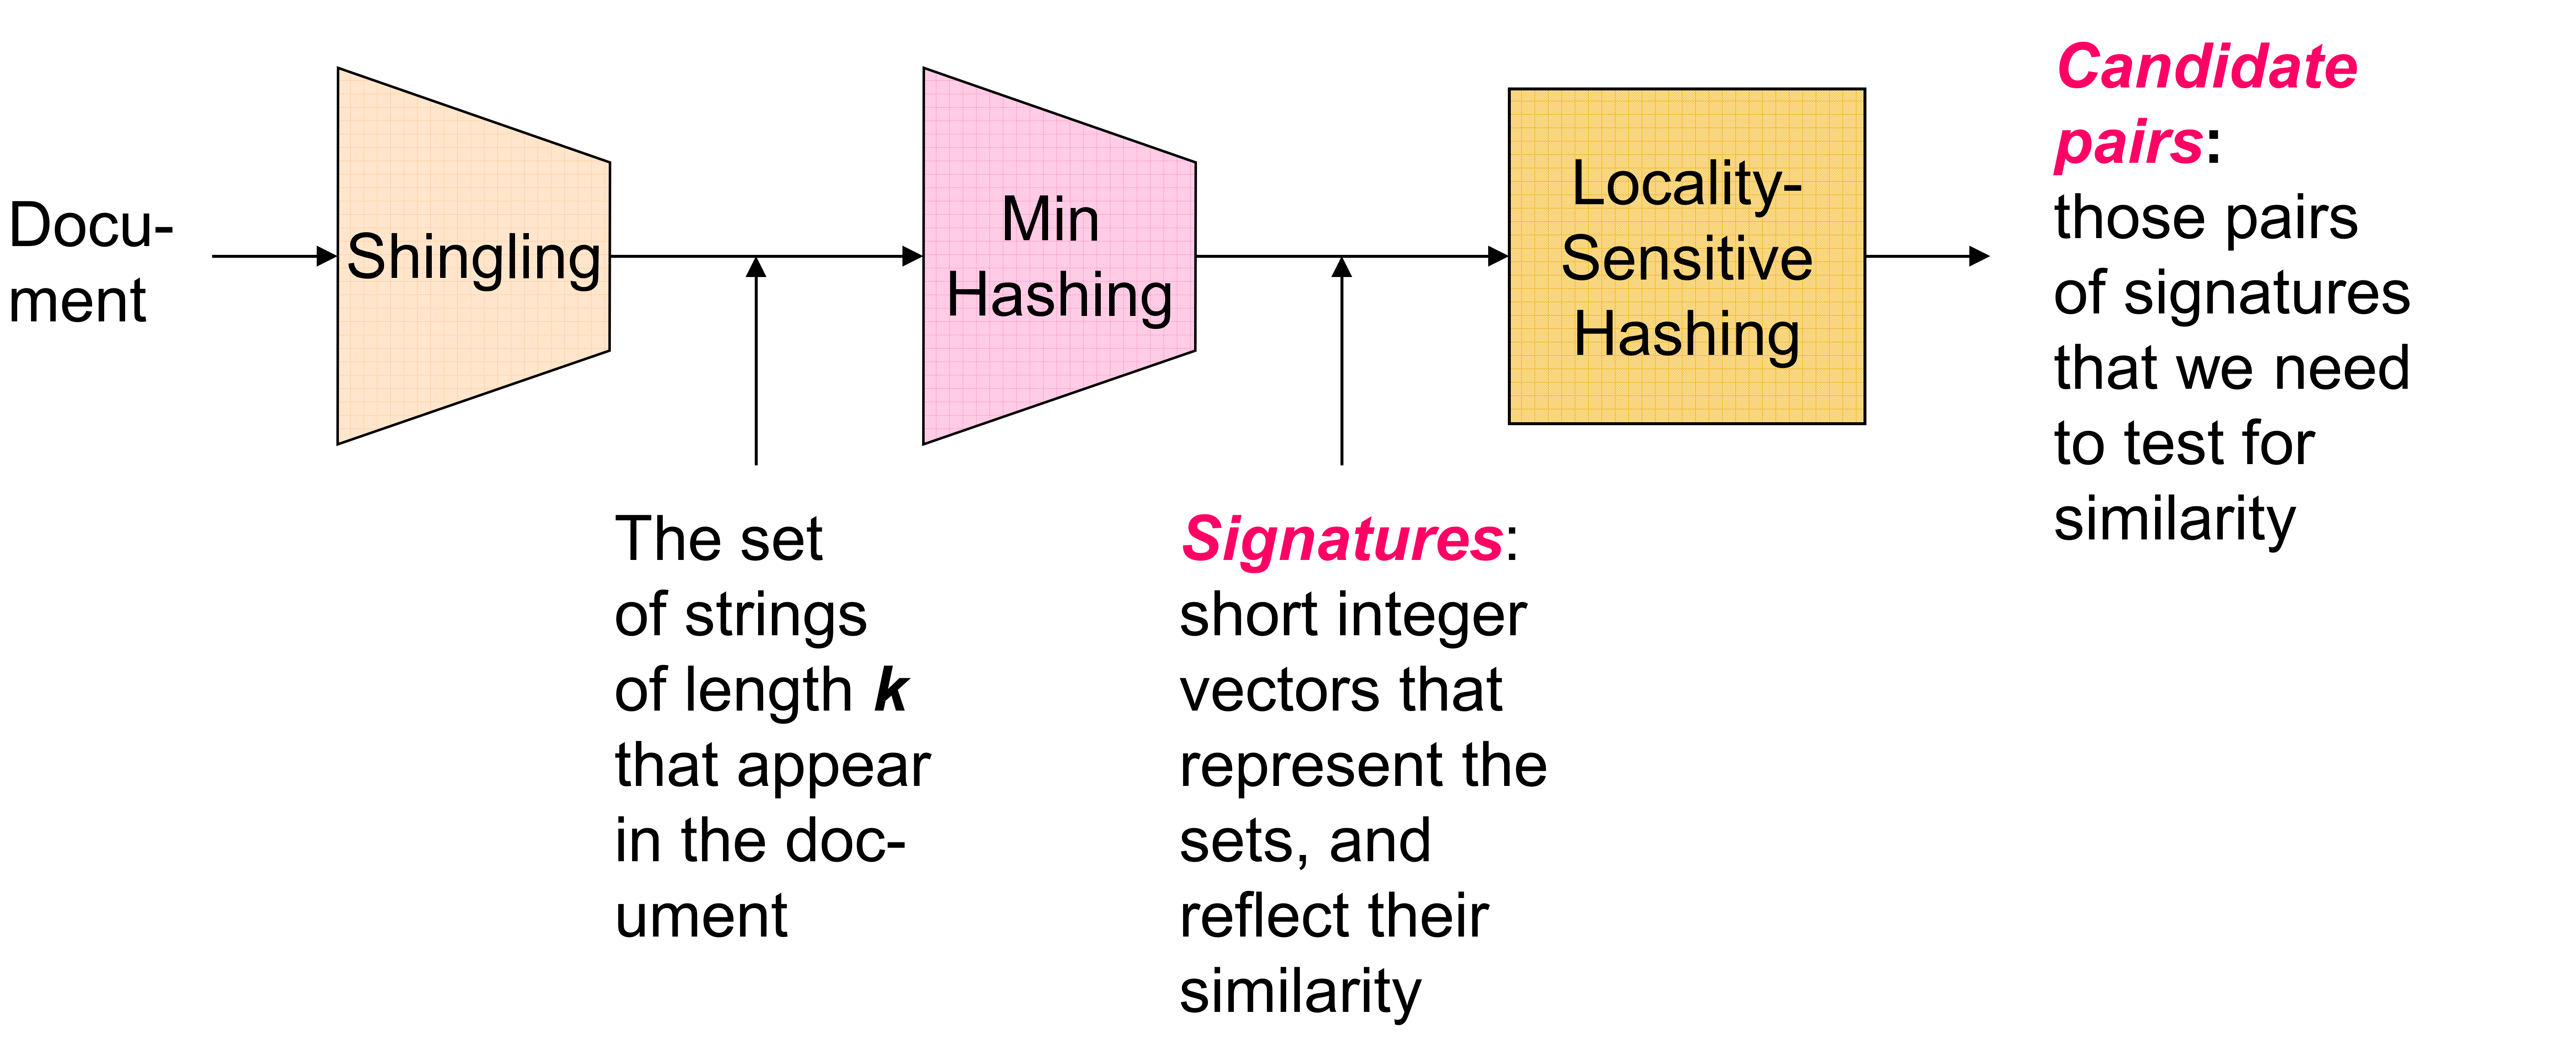
\includegraphics[scale = 0.4]{images//RoughFlow.png}
			\caption*{\textbf{Source:} J. Leskovec, A. Rajaraman, J. Ullman: Mining of Massive Datasets}
			\end{center}
		\end{figure}
	\end{frame}
%%%%%%%%%%%%%%%%%%%%%%%%%%%%%%%%%%%%%%%%%%%%%%%%%%%%%%%%%%%%%%%%%%%%%%%%%%%%%%%%%%%%%%%%%%%%%%%%%%%%%%%%%%%%%%%%%%%%%%%%%%%%%%%%%%%%%%%%%%%%%%%%%%%%%%%%%%%%%%%%%%%%%%%%%%%%%%%%%%%%%%%%%%%%%%%%%%%
\begin{frame}
		\frametitle{Jaccard Similarity } 
		\begin{itemize}[topsep=0pt,itemsep=0ex,partopsep=1ex,parsep=1ex]
			\item [$\square$] \textbf{Jaccard Similarity:} Let S1 and S2 are two sets, then jaccard similarity between two sets  is defined as
			\pause
			$$ \text{SIM(S1,S2)} = \dfrac{|S1 \cap S2|}{|S1 \cup S2|} $$
		\end{itemize}
	\end{frame}


\begin{frame}
		\frametitle{Shingling} 
		\begin{itemize}[topsep=0pt,itemsep=0ex,partopsep=1ex,parsep=1ex]
			\item [$\square$] \textbf{Shingling:} Shingling convert documents to sets.
			\item [$\square$] \textbf{k-shingle:} A k-shingle is consecutive sub-string of k-words(or k-characters) of the document string. The alternate name for k-shingle is k-gram.
			\item [$\square$] \textbf{Example:} If $D1$ and $D2$ two sets, 
			\item $\bm{D1:}$ De duplication  Using Locality Sensitive Hashing
			\item $\bm{D2:}$ Using Locality Sensitive Hashing for De duplication
			
		\end{itemize}
\end{frame}

\begin{frame}
		\frametitle{Shingling} 
		\begin{itemize}[topsep=0pt,itemsep=0ex,partopsep=1ex,parsep=1ex]
			\item [$\square$] $\bm{D1}$ = \{“De duplication”, “duplication Using”, “Using Locality”, “Locality Sensitive”, “Sensitive
				Hashing”\} \\
			\item [$\square$] $\bm{D2}$ = \{“Using Locality”, “Locality Sensitive”, “Sensitive Hashing”, “Hashing for”, “for De”, “De duplication”\} 
			\item [$\square$] $\bm{D1 \cap D2}$ = \{“De duplication’, “Using Locality”, “Locality Sensitive”, “Sensitive Hashing”\}  
			\item [$\square$] $\bm{D1 \cup D2}$ = \{“De duplication”, “duplication Using”, “Using Locality”, “Locality Sensitive”, “Sensitive Hashing”, “Hashing for”, “for De”\}
			\item	$$ \bm{	SIM(D1,D2) = \frac{|D1 \cap D2|}{|D1 \cup D2|} = \frac{4}{7} = 0.57} $$
		\end{itemize}
\end{frame}
%------------------------------------------------
\begin{frame}
\frametitle{Characteristic Matrix Corresponding to Documents}
	\begin{itemize}
			\item [$\square$] For above two document sets $D1$ and $D2$ the characteristic matrix is as follow
	\end{itemize}
	\pause
	\begin{table}[H]
		\begin{center}
%			\setstretch{1.5}
			\begin{tabular}{|c|c|c|}
			\hline
			$\bm{D1 \cup D2}$ &$\bm{ D1}$ &$\bm{ D2}$\\
			\hline
			``De duplication"&1 & 1 \\
			\hline
			``duplication Using"& 1  & 0 \\
			\hline
			``Using Locality" & 1 & 1\\
			\hline
			``Locality Sensitive"&1 & 1\\
			\hline
			``Sensitive Hashing"& 1 & 1 \\
			\hline
			``Hashing for"& 0 & 1 \\
			\hline
			``for De"& 0 & 1 \\
			\hline
			\end{tabular}
		\end{center}
	\end{table}
\end{frame}


\begin{frame}
\frametitle{Min-Hashing}
\begin{itemize}[topsep=0pt,itemsep=0ex,partopsep=1ex,parsep=1ex]
\item [$\square$] The aim of min-hashing is to convert large sets to short signatures, while preserving similarity.
\item [$\square$] Suppose the rows of the boolean matrix permuted under random permutation $\bm{\pi}$
\item [$\square$] Define a \textbf{hash} function $\bm{h_{\pi}(C)}$ = the index of the first (in the permuted order $\bm{\pi}$) row in which column $\bm{C}$ has value $\bm{1}$:
			$$ \bm{h_{\pi}(C)  = min_{\pi}\pi(C) }$$

\end{itemize}
\end{frame}

\begin{frame}
		\frametitle{Example of Signature Matrix}
		\pause
     	\vspace*{1cm}
		\begin{figure}[H]
			\begin{center}
			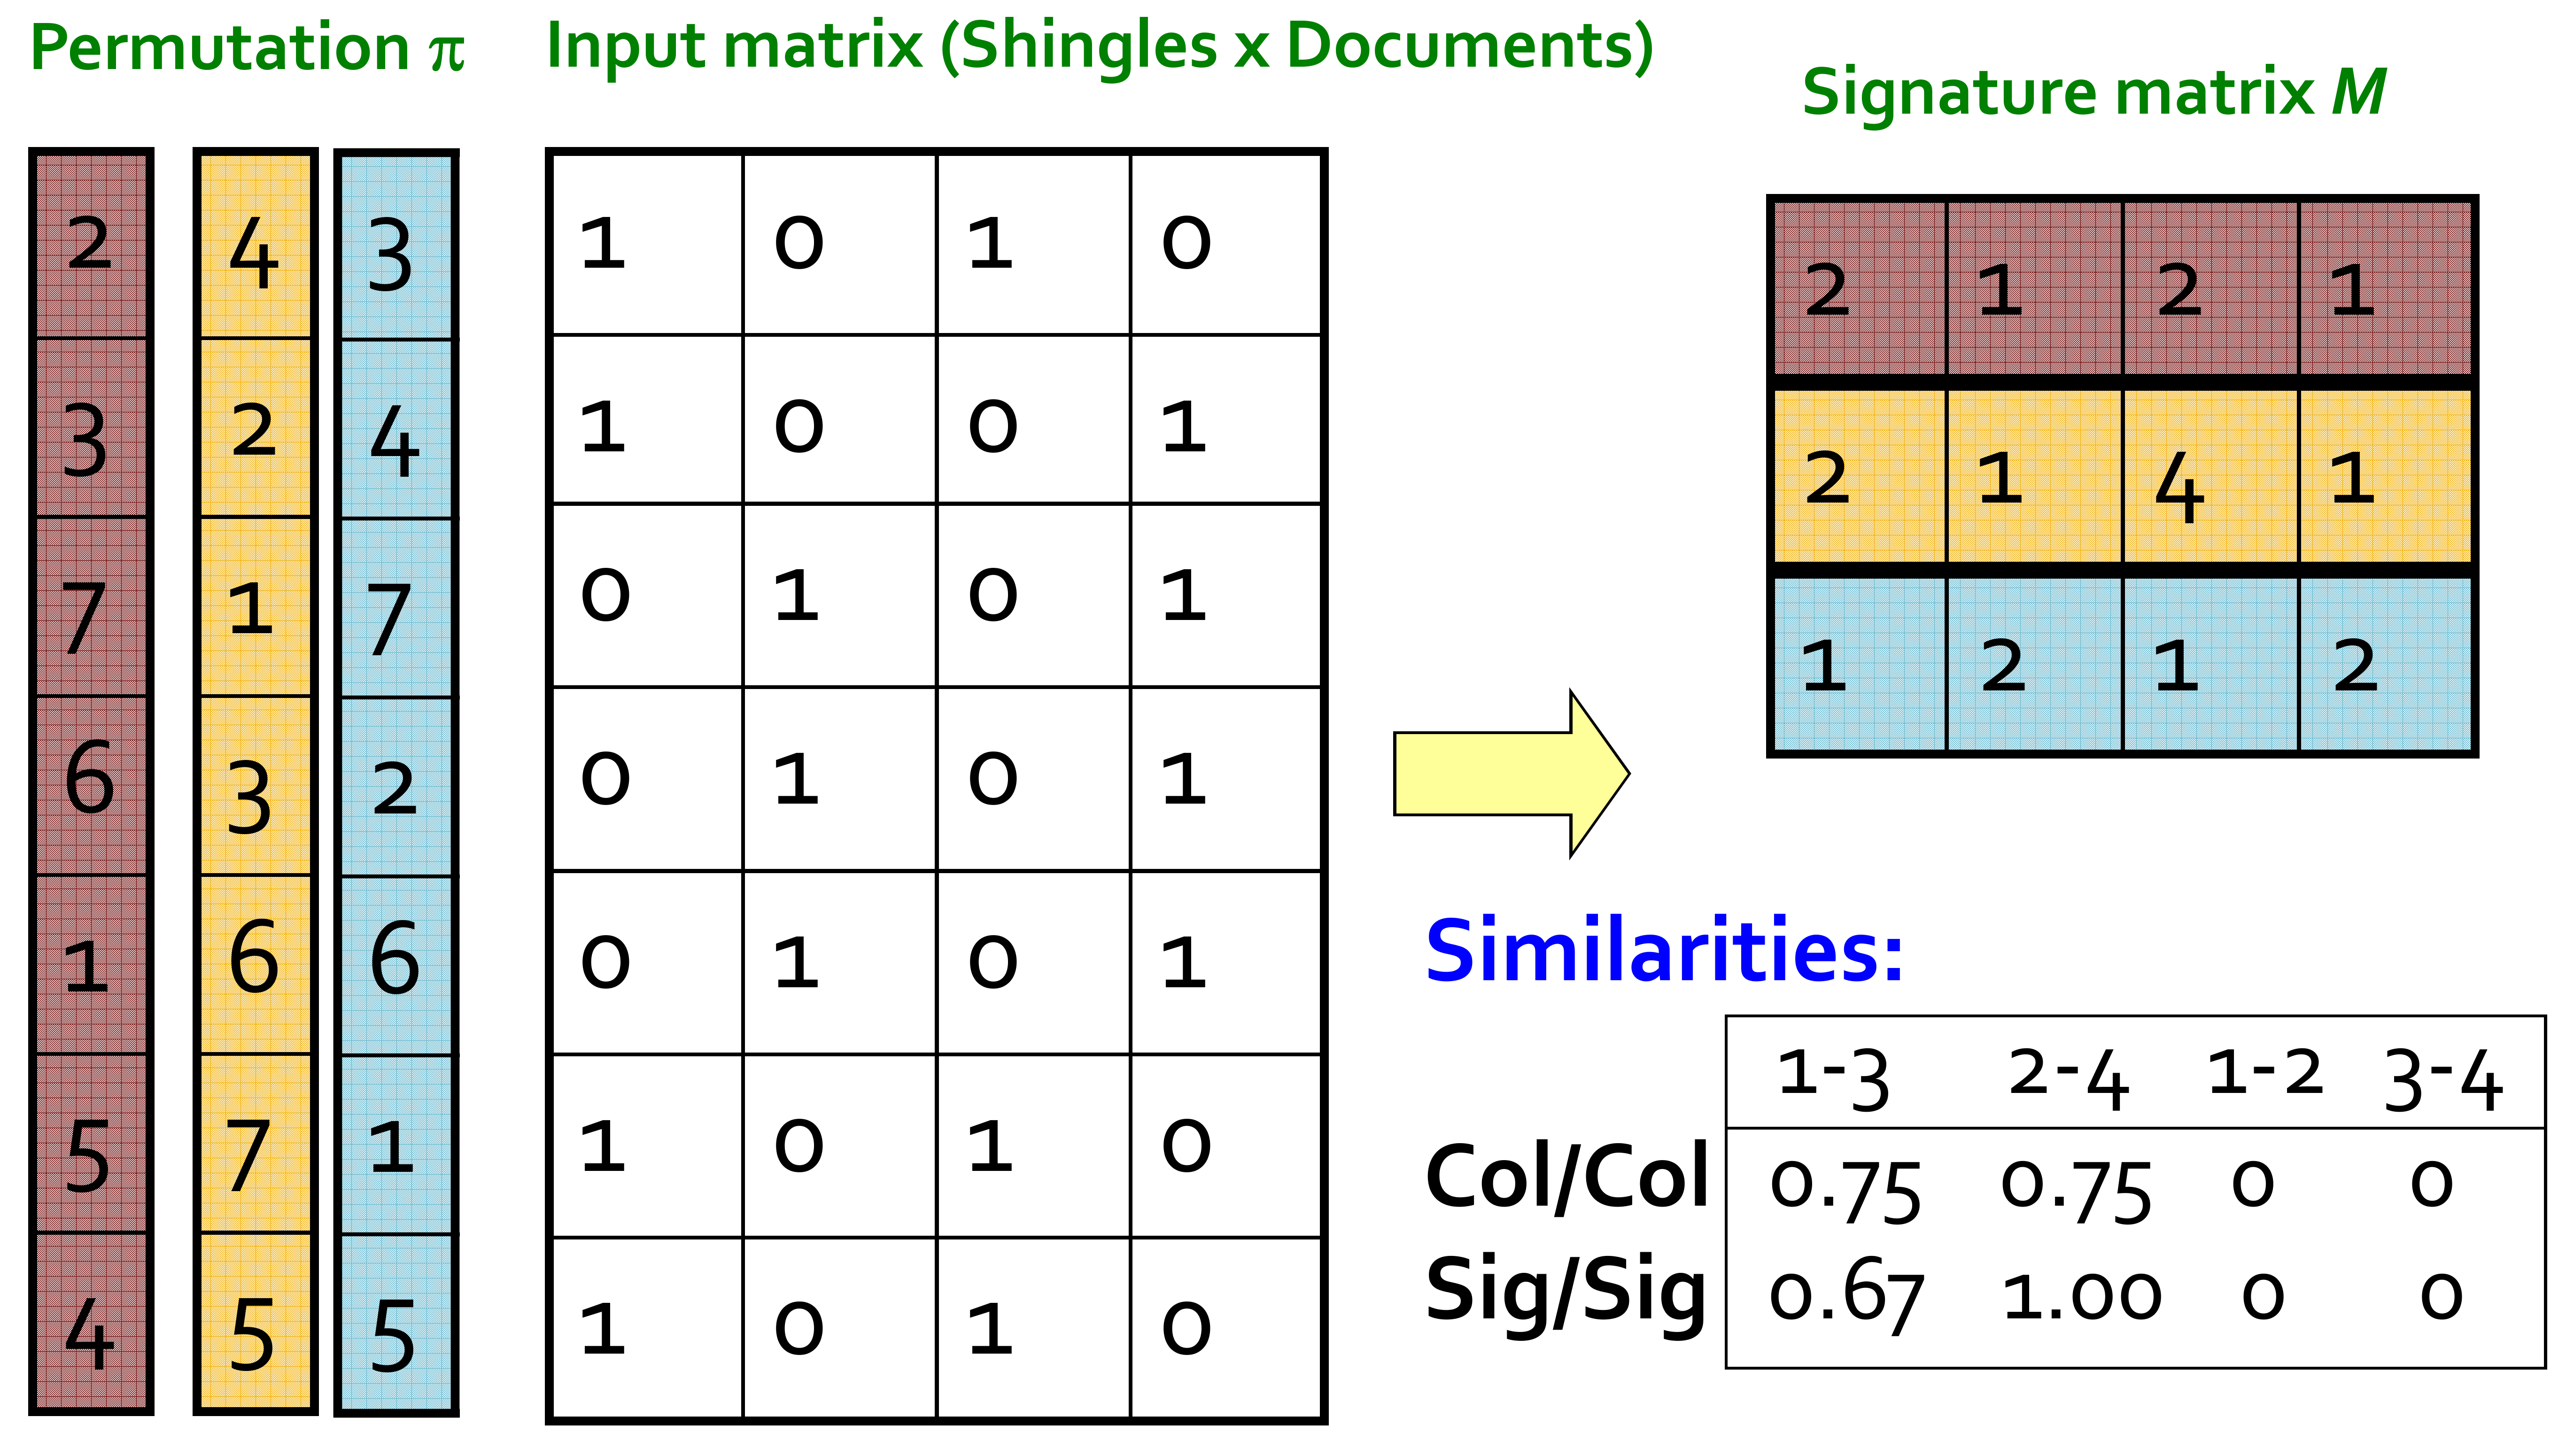
\includegraphics[scale = 0.4]{images//signature.png}
			\caption*{\textbf{Source:} J. Leskovec, A. Rajaraman, J. Ullman: Mining of Massive Datasets}
			\end{center}
		\end{figure}
\end{frame}

\begin{frame}{Locality Sensitive Hashing}
\begin{itemize}[topsep=0pt,itemsep=0ex,partopsep=1ex,parsep=1ex]
\item [$\square$] The basic idea of locality sensitive hashing to use a function f(x,y) that tells whether x and y is a candidate pair(i.e. a pair of elements whose similarity must be evaluated).
\item [$\square$] \textbf{Method to find such $\bm{f}$ from Min-hash Signature matrix:}
\begin{enumerate}
\item [$\square$] Divide the rows of signature matrix in $b$ band having $r$ rows.
\end{enumerate}
\end{itemize}
\pause
\begin{figure}[H]
\begin{center}
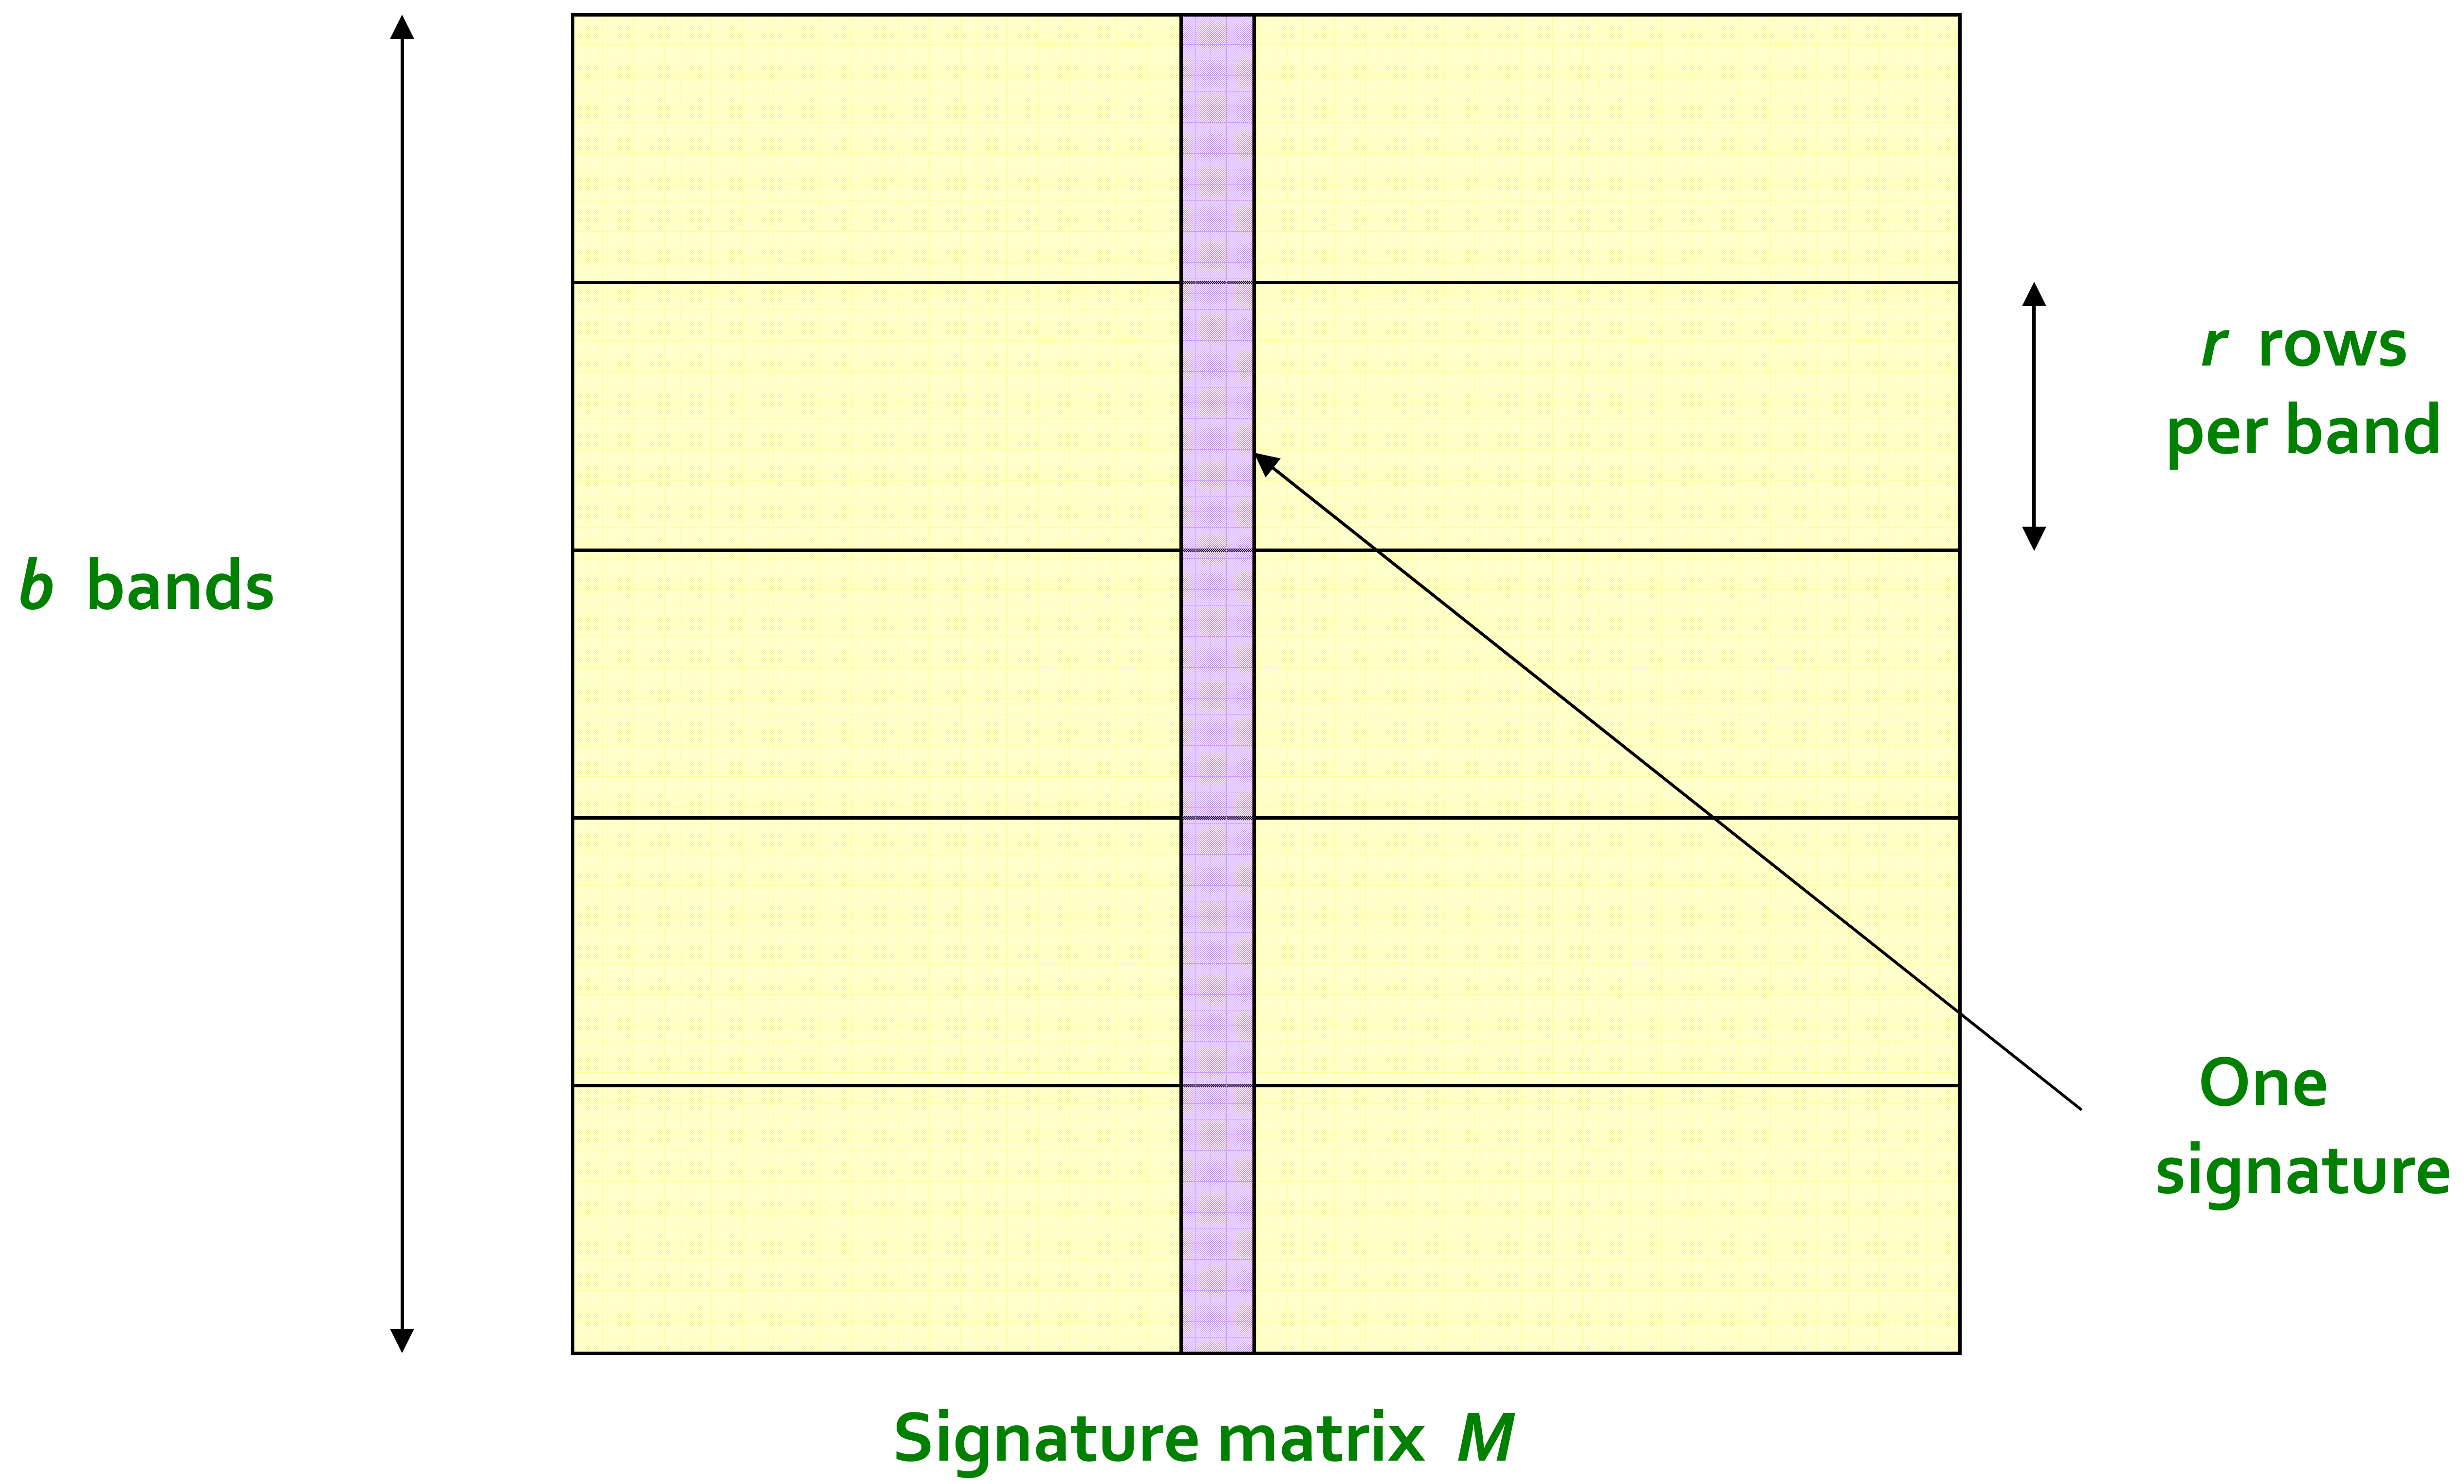
\includegraphics[scale = 0.3]{images//bands.png}
\caption*{\textbf{Source:} J. Leskovec, A. Rajaraman, J. Ullman: Mining of Massive Datasets}
\end{center}
\end{figure}
\end{frame}

\begin{frame}{Locality Sensitive Hashing}
\begin{itemize}[topsep=0pt,itemsep=0ex,partopsep=1ex,parsep=1ex] 
\item 
\begin{enumerate}
\item [$\square$] For each band hash the column in k buckets, buckets contains column pairs if there are identical in particular band and the pair of a bucket are called \textbf{candidate pairs}
\end{enumerate}
\end{itemize}
\pause 
\begin{figure}[H]
\begin{center}
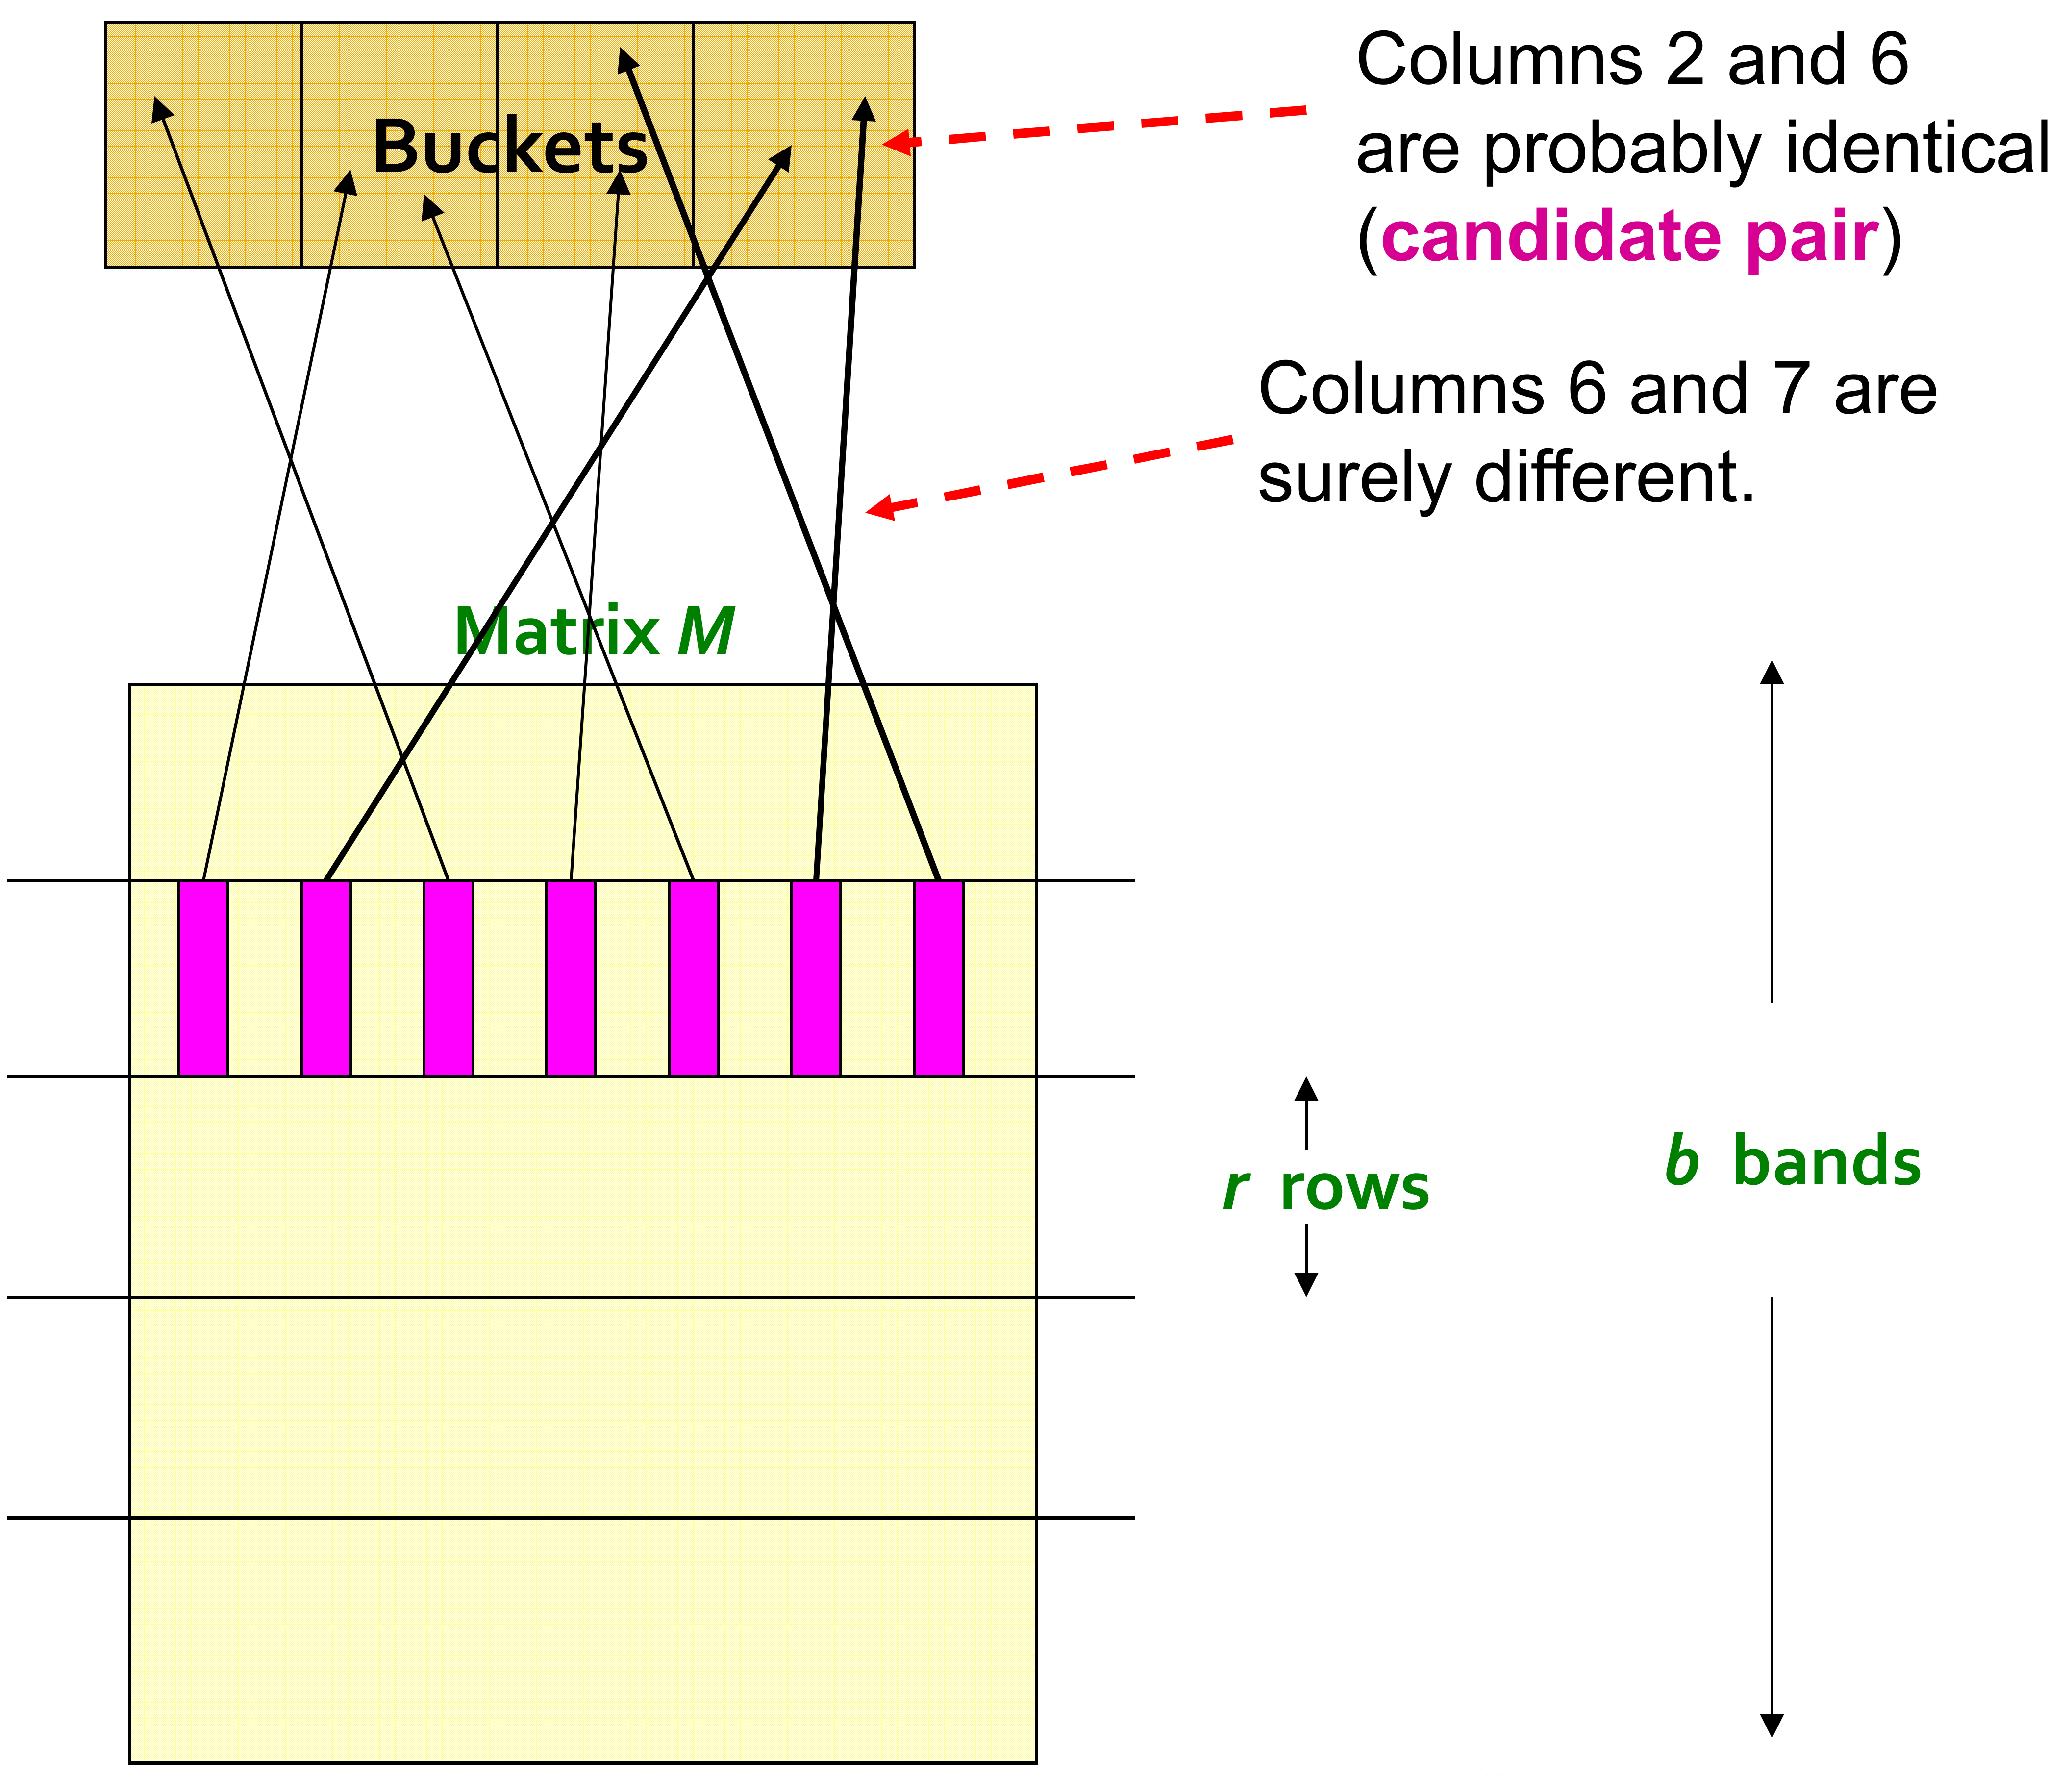
\includegraphics[width= 8cm, height=5cm]{images//buckets.png}
\caption*{\textbf{Source:} J. Leskovec, A. Rajaraman, J. Ullman: Mining of Massive Datasets}
\end{center}
\end{figure}
\end{frame}

\begin{frame}{Interpretation of b bands for r rows:}
\begin{itemize}
\item [$\square$] We want that for column whose similarity is greater than threshold t will goes to same bucket with probability 1 .
\begin{figure}[H]
\begin{center}
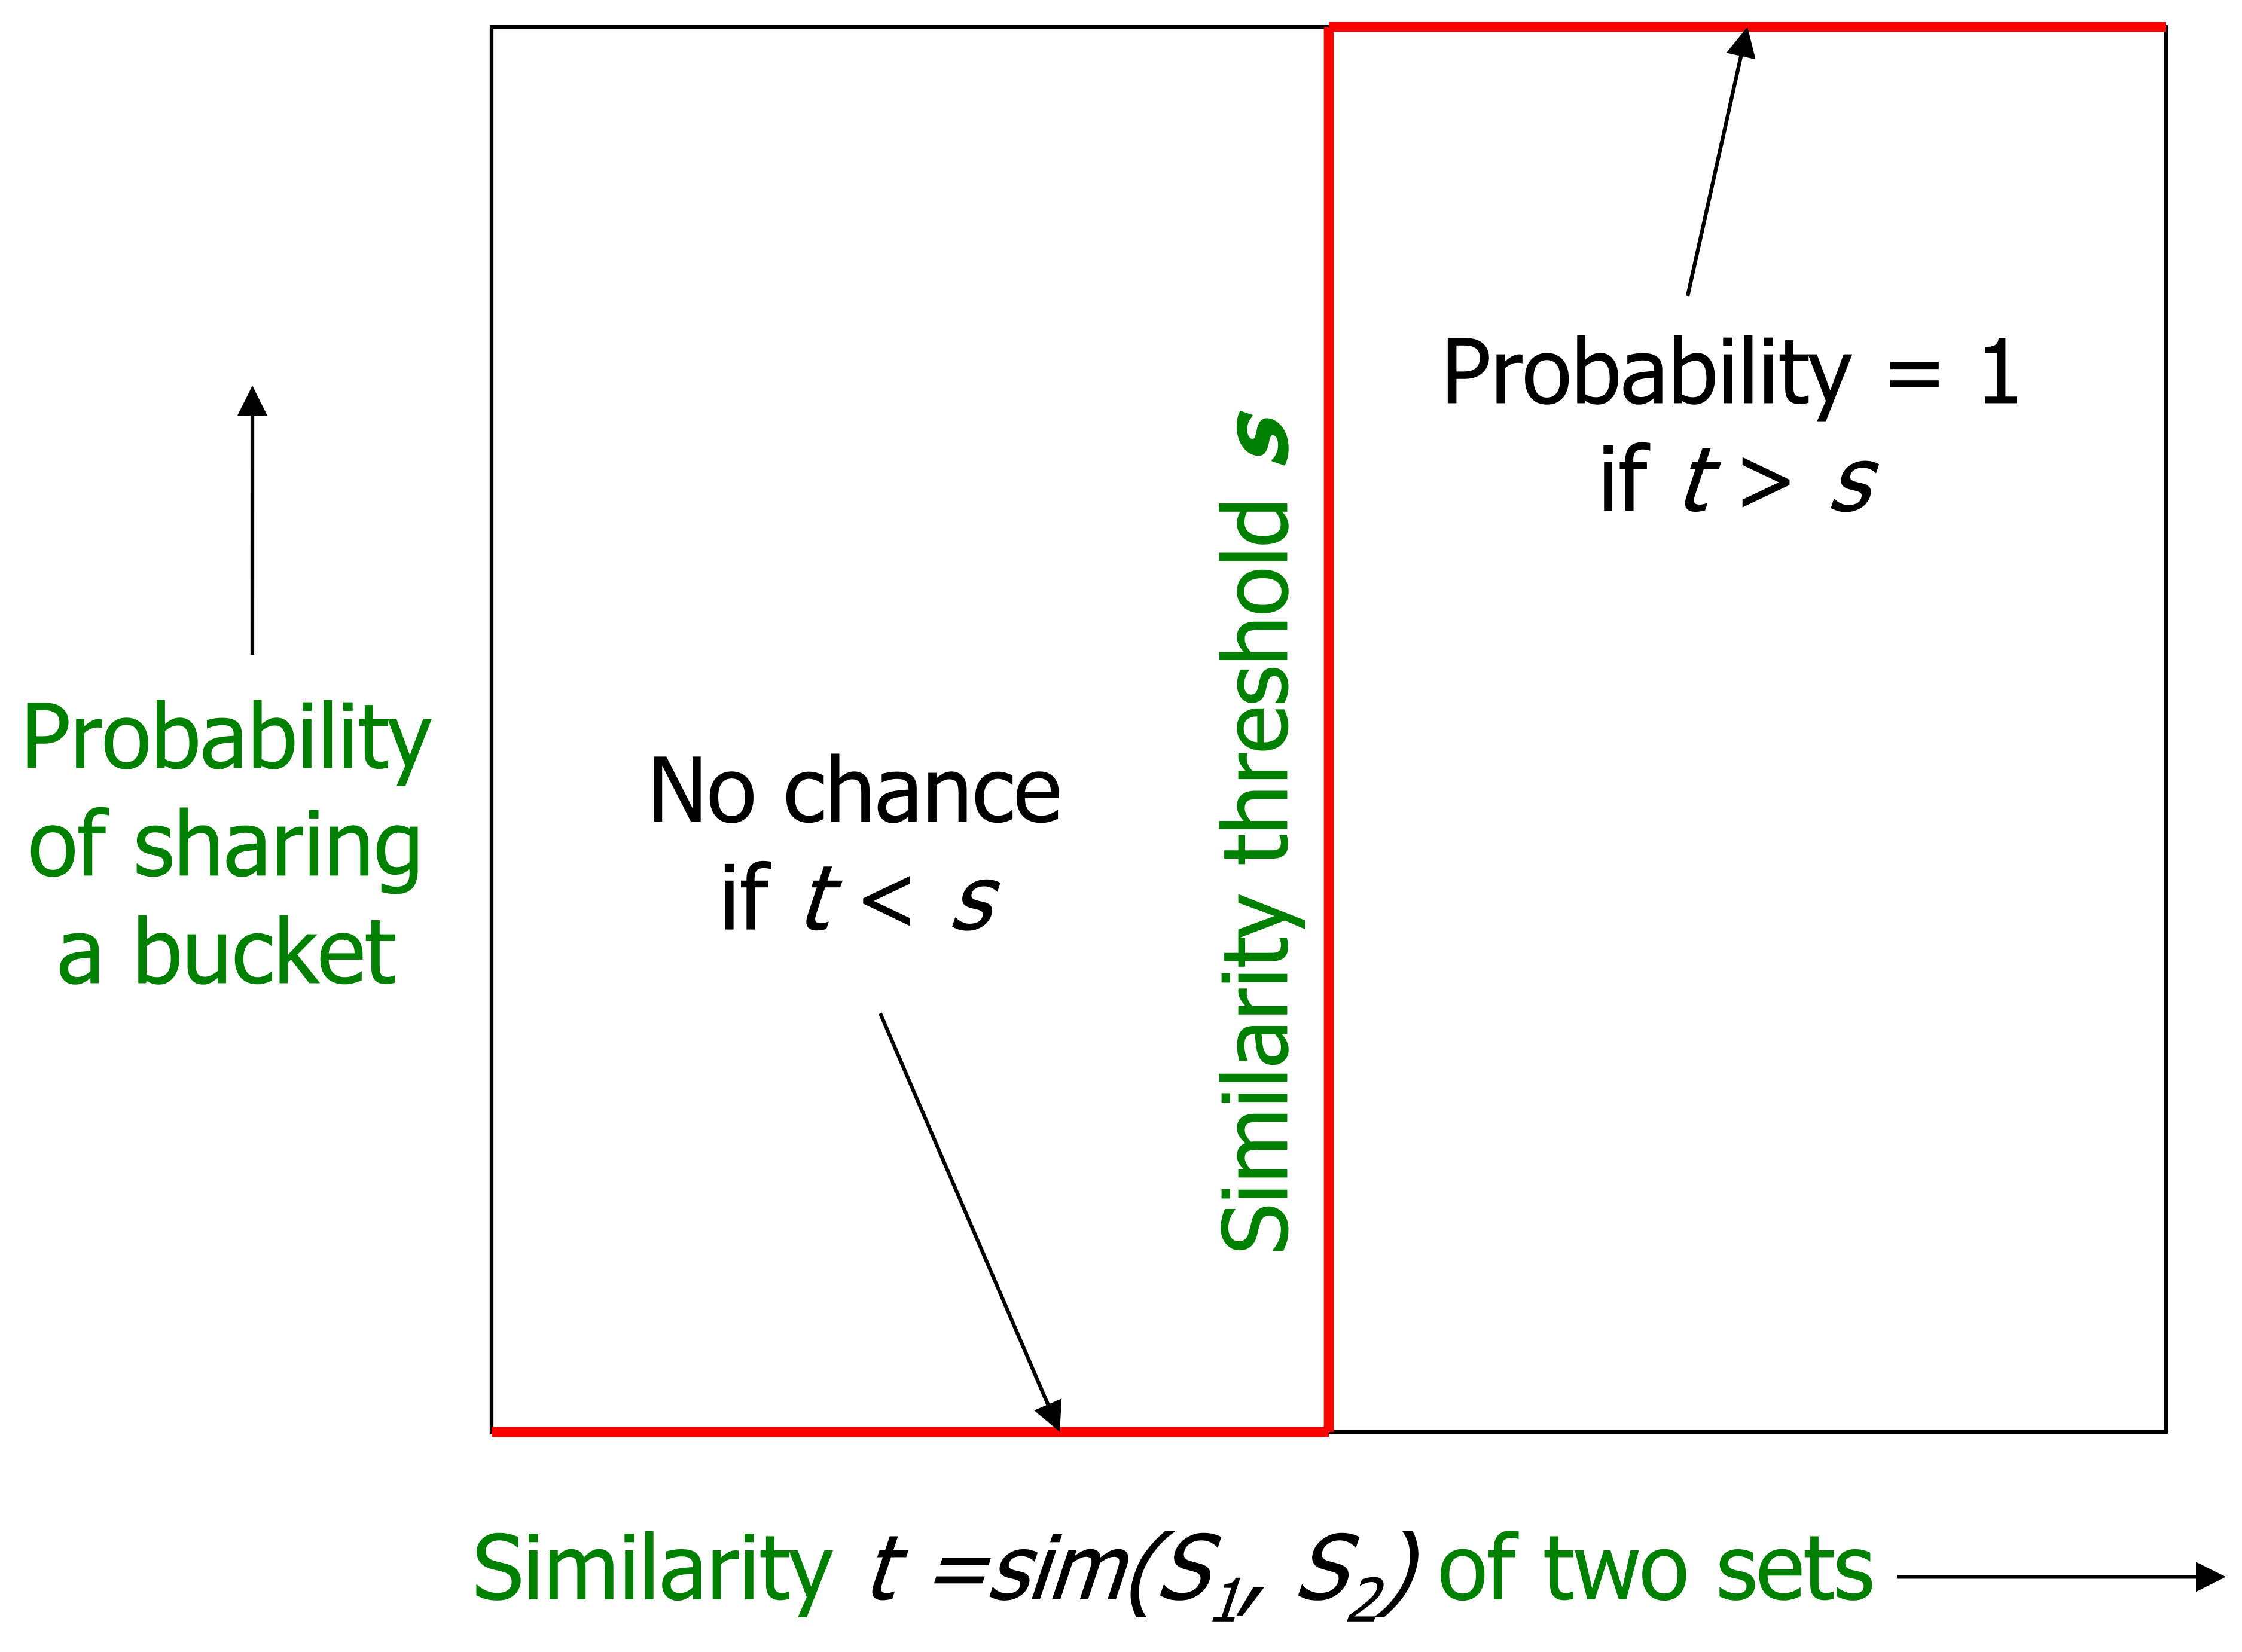
\includegraphics[scale = 0.5]{images//img1.png}
\caption*{\textbf{Source:} J. Leskovec, A. Rajaraman, J. Ullman: Mining of Massive Datasets}
\end{center}
\end{figure}
\end{itemize}
\end{frame}

\begin{frame}{Interpretation of b bands for r rows:}
\begin{itemize}
\item [$\square$] For $b = 1$ and $r = 1$:
\begin{figure}[H]
\begin{center}
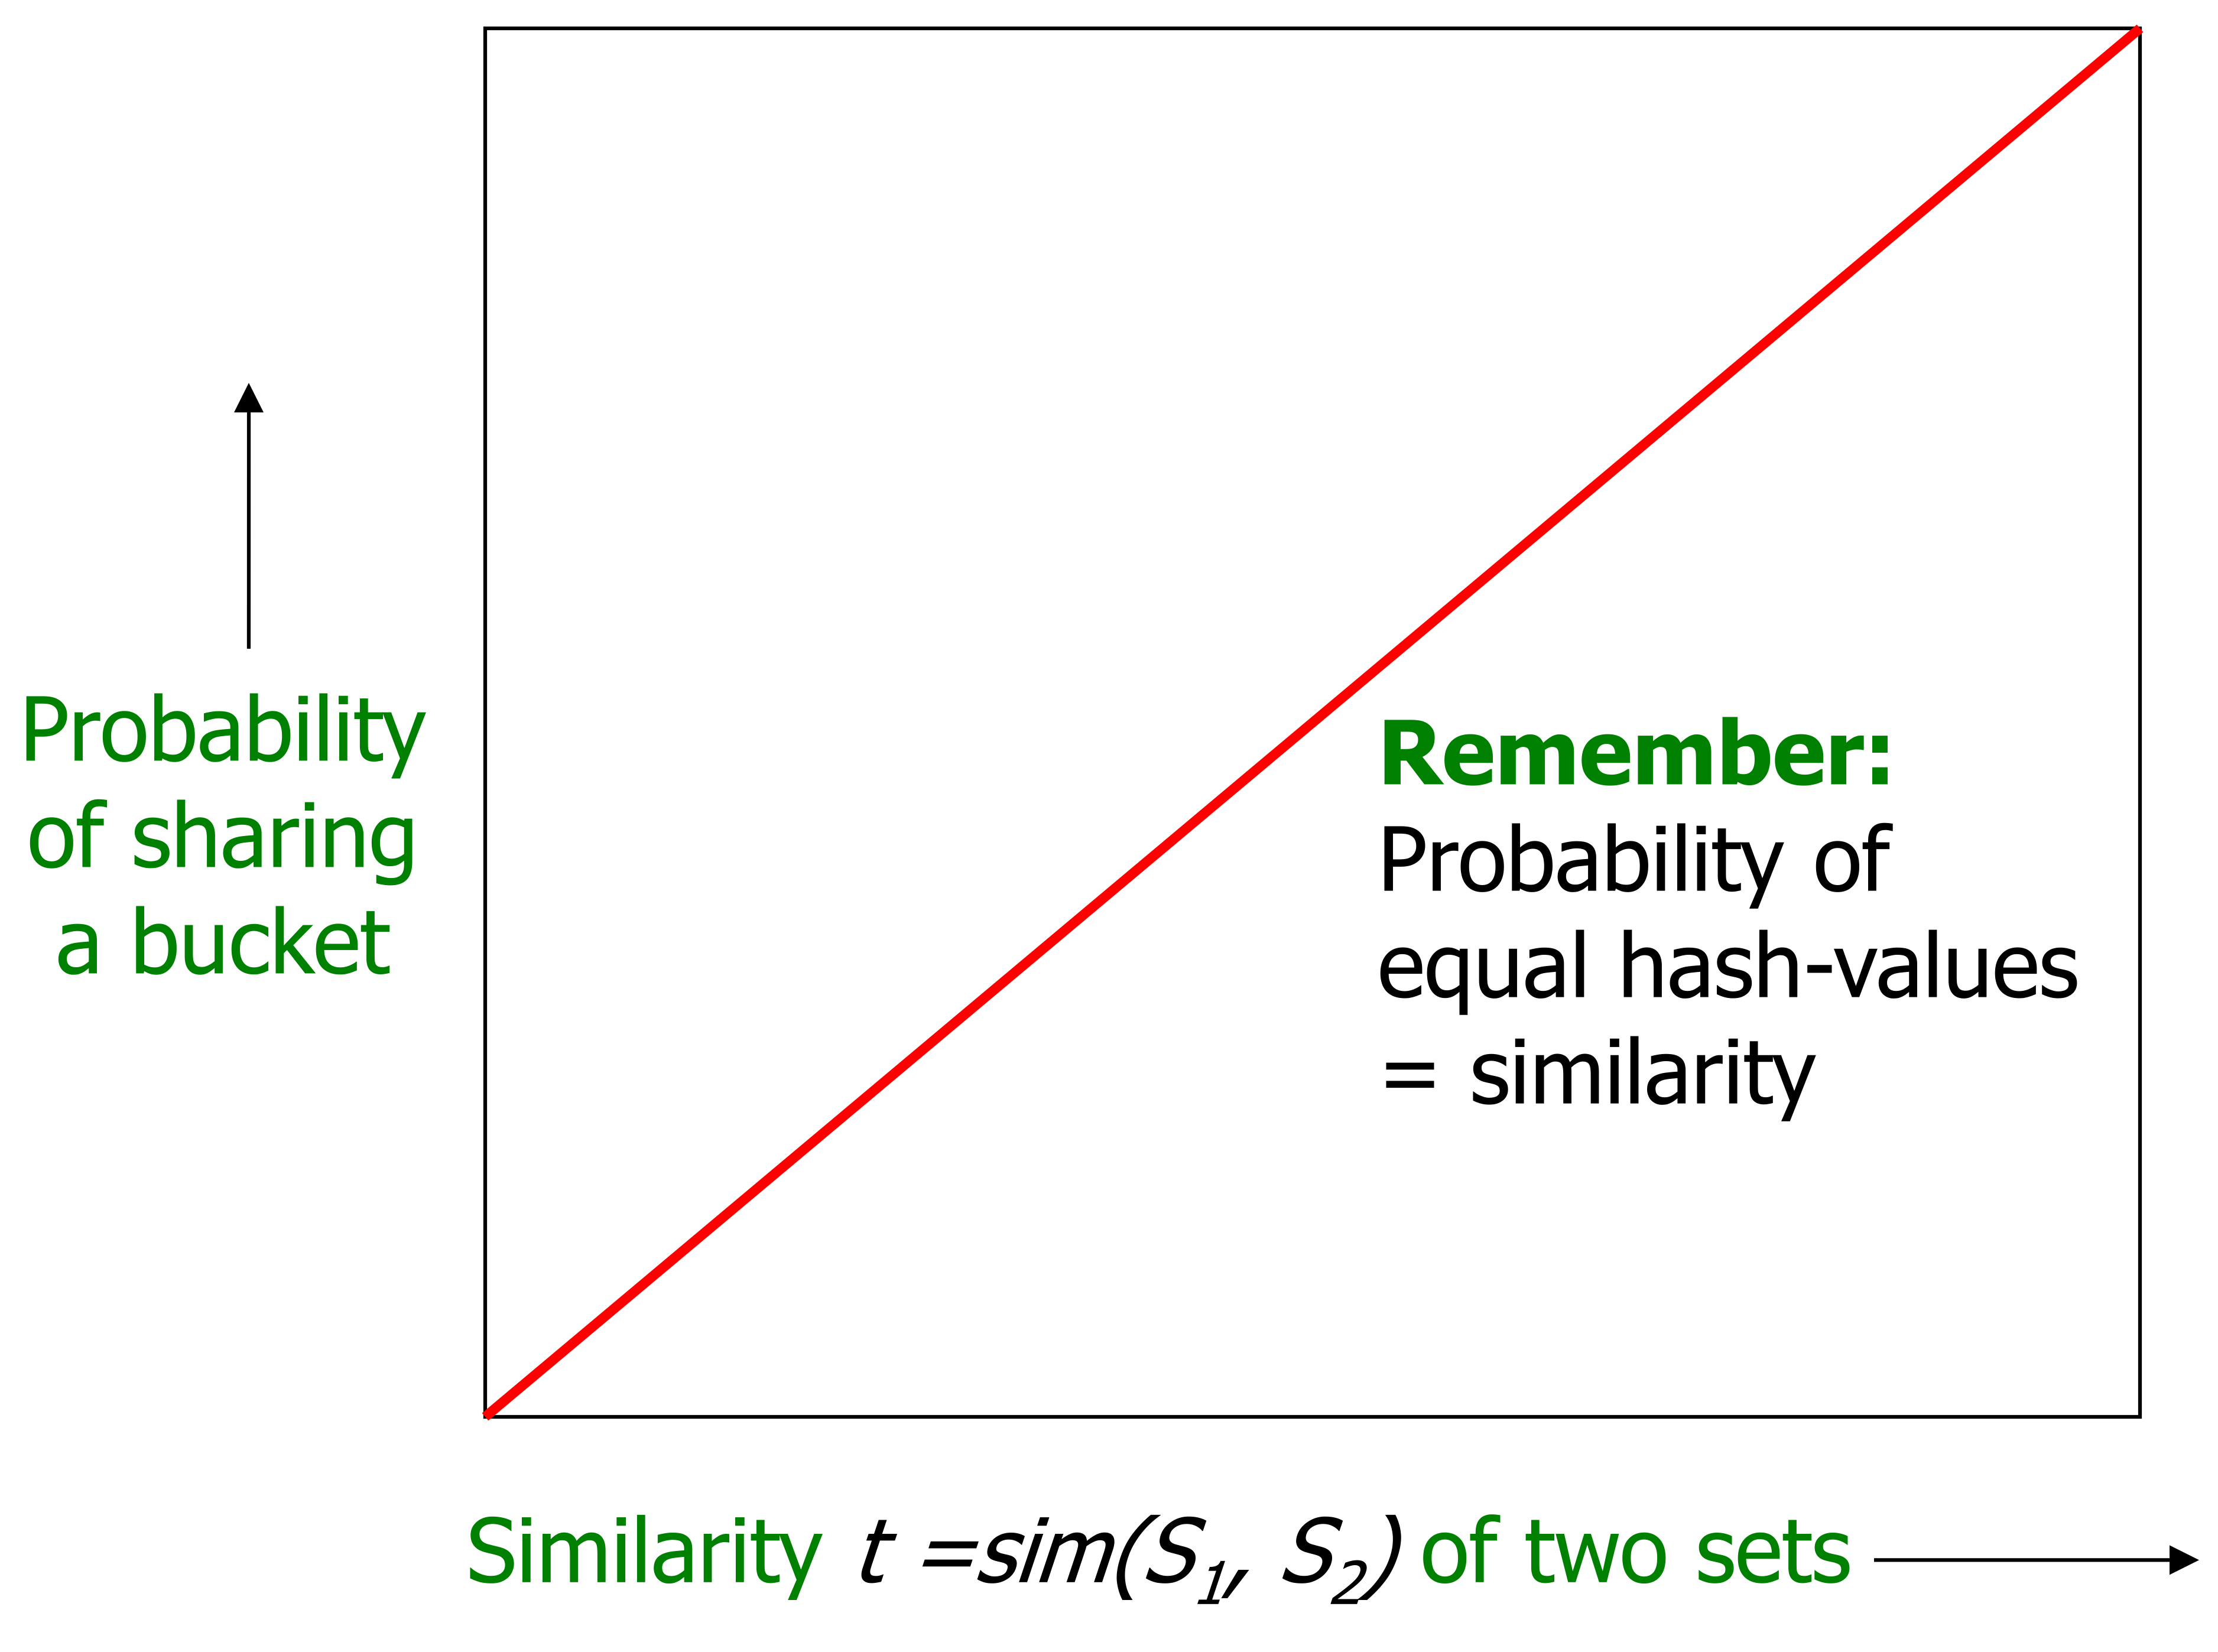
\includegraphics[scale = 0.5]{images//img2.png}
\caption*{\textbf{Source:} J. Leskovec, A. Rajaraman, J. Ullman: Mining of Massive Datasets}
\end{center}
\end{figure}
\end{itemize}
\end{frame}

\begin{frame}{Interpretation of b bands for r rows:}
\begin{itemize}
\item [$\square$] For $b$ bands and $r$ rows:
\begin{figure}[H]
\begin{center}
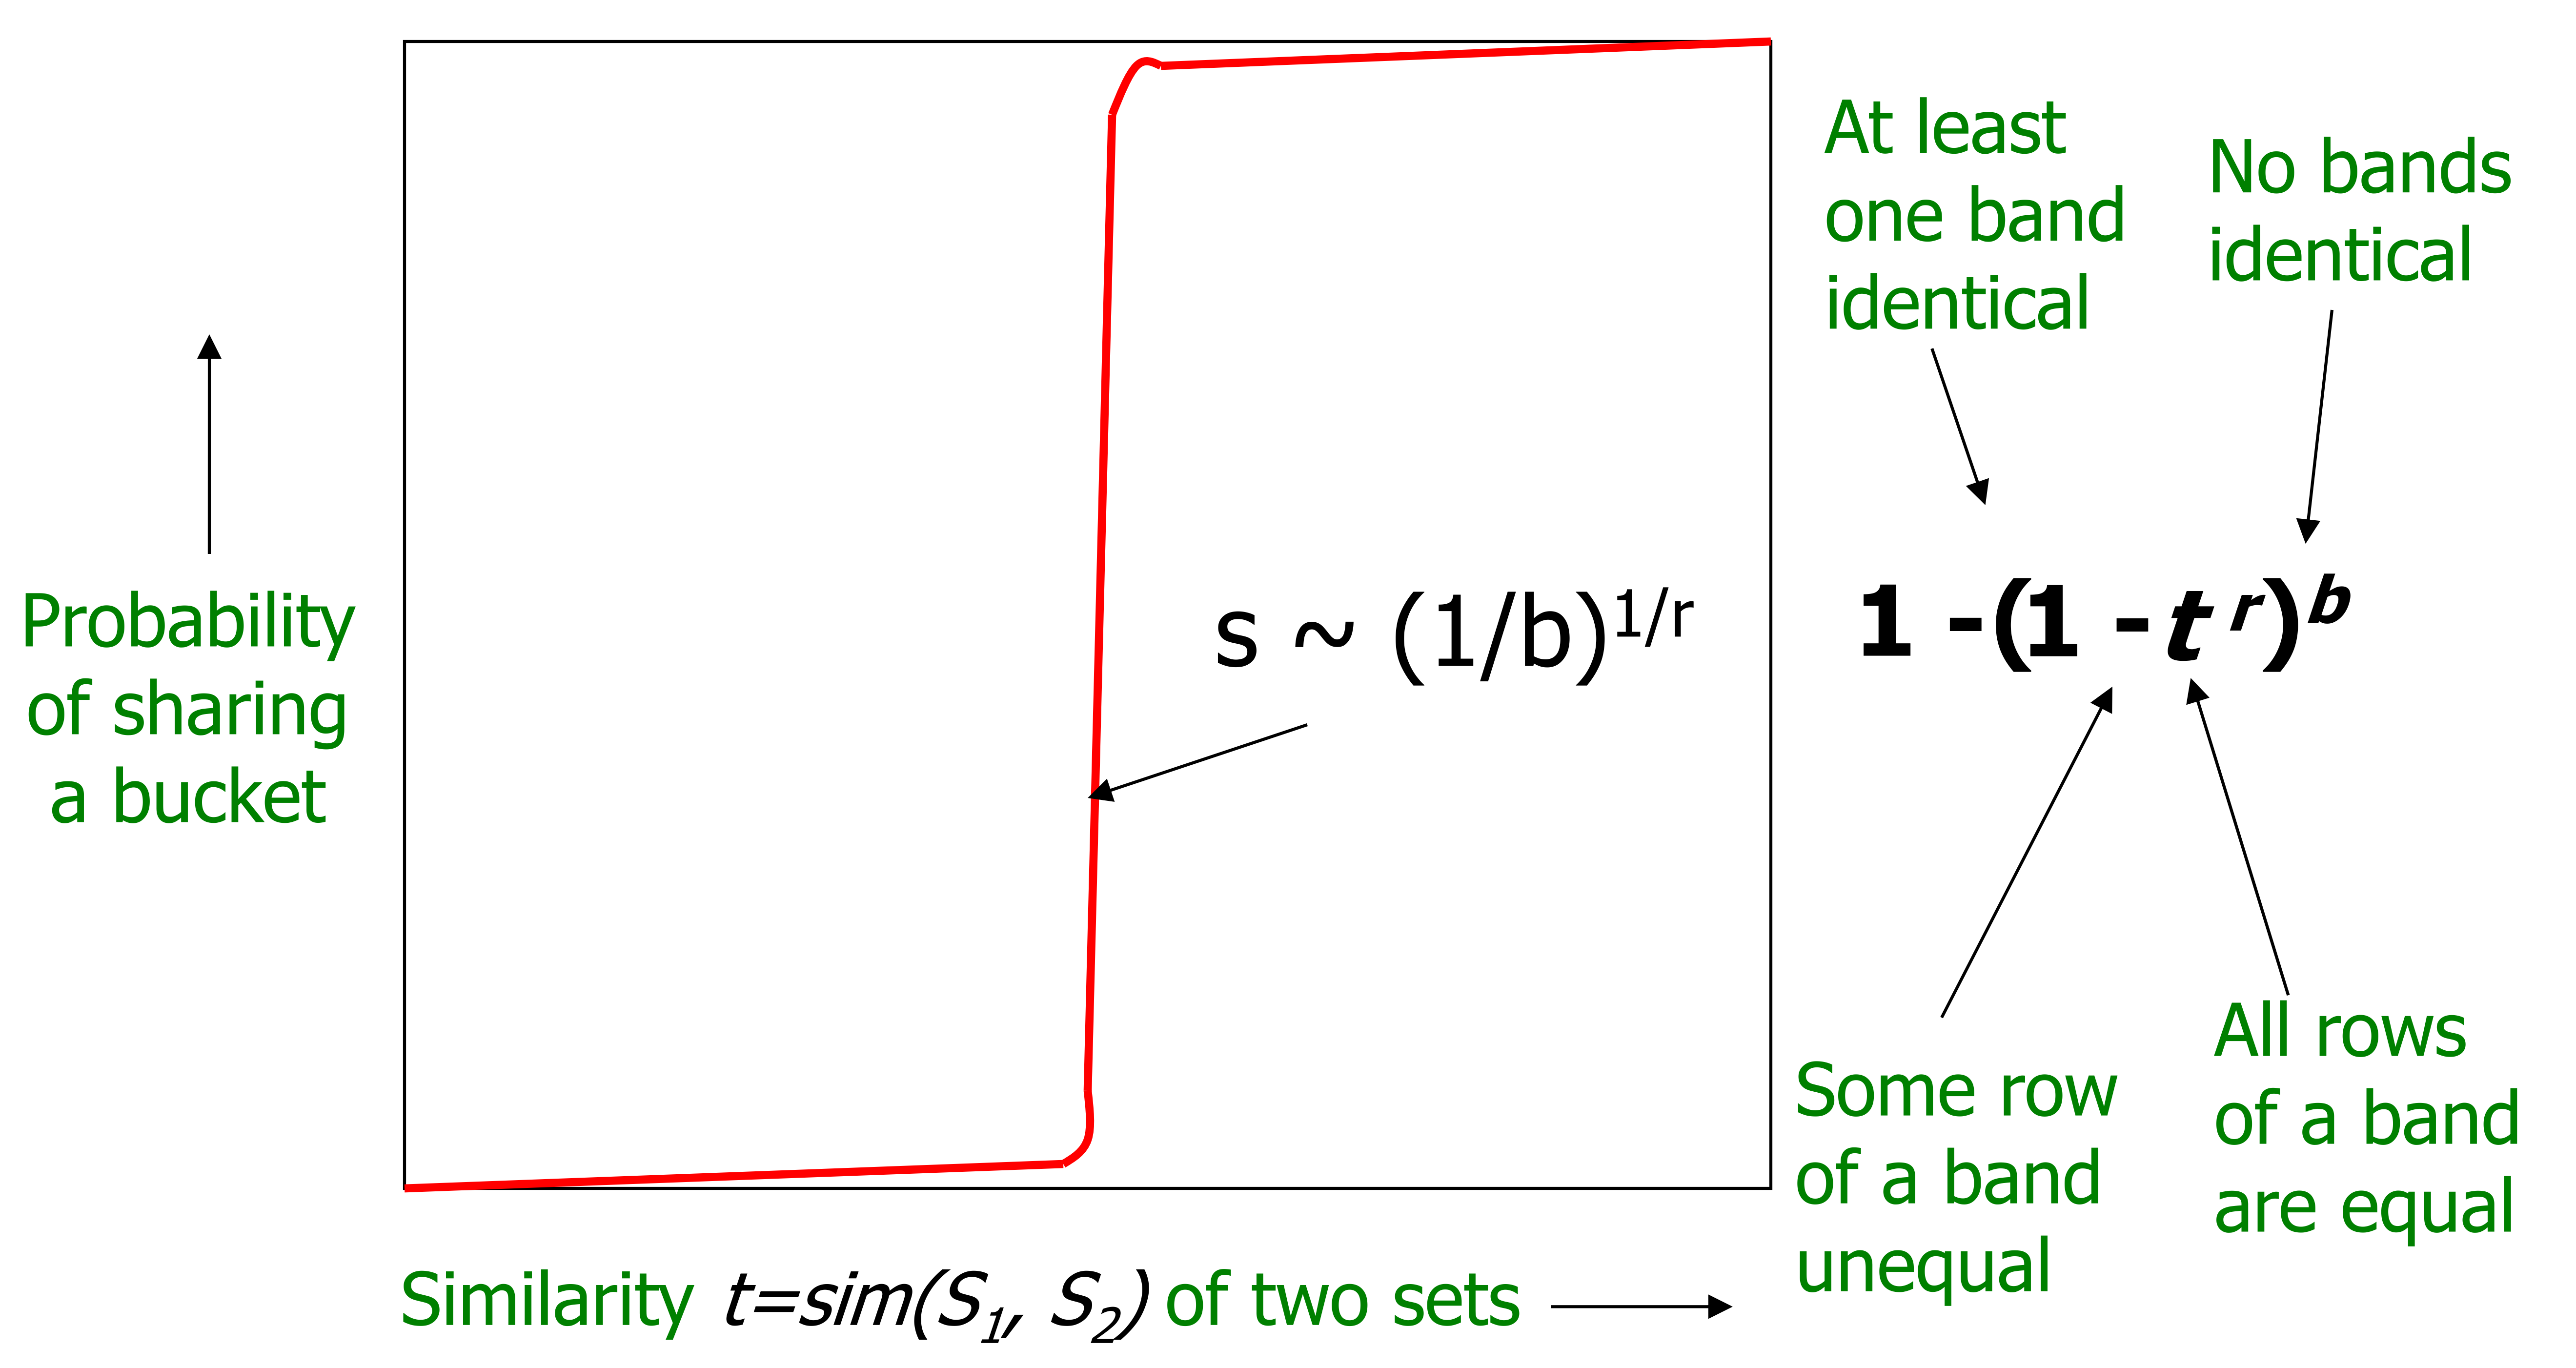
\includegraphics[scale = 0.5]{images//img3.png}
\caption*{\textbf{Source:} J. Leskovec, A. Rajaraman, J. Ullman: Mining of Massive Datasets}
\end{center}
\end{figure}
\end{itemize}
\end{frame}


\begin{frame}{Results}
\begin{itemize}
\item [$\square$] To check the Working and performance of the implemented locality sensitive hashing algorithm, \textbf{20 Newsgroup} text data set containing $600$ hundred text files is taken in consideration.
\item [$\square$] The actual truth about the data set is not known, we computed the jaccard similarity of all combinations of text files, and those having jaccard similarity greater than $0.55$, kept in same cluster.
\item [$\square$] We found $8$ such clusters and are as follow:
\end{itemize}
\pause
\scalefont{0.8}
\begin{table}[H] \label{table1}
\begin{center}
%\setstretch{1.5}
\caption{Actual Truth}
\begin{tabular}{|c|c|}
\hline
Cluster Number & File ID's\\
\hline
1              & \textbf{[51150, 51240]} \\
2              & \textbf{[51270, 51307]}\\
3              & \textbf{[53072, 53178]}\\
4              & \textbf{[37917, 37950]}\\
5              & \textbf{[38216, 38255]}\\
6              & \textbf{[38227, 38330]}\\
7              & \textbf{[38320, 38432]}\\
8              & \textbf{[38438, 38442, 38458]}\\
\hline
\end{tabular}
\end{center}
\end{table}
\end{frame}

\scalefont{1}
\begin{frame}{Results}
\begin{itemize}
\item [$\square$] k (for k-shingle) = 5
\item [$\square$] Total number of hash functions for Min-hashing = 100
\item [$\square$] Number of bands ($b$) = 10
\item [$\square$] Number of rows in a band  ($r$) = 6
\end{itemize}
\pause
\begin{table}[H] 
\label{table2}
\begin{center}
\scalefont{0.9}
\caption{Predicted Duplicates}
\begin{tabular}{|c|c|}
\hline
Cluster Number & File ID's \\
\hline
\textcolor{azure}{1}             & \textcolor{azure}{\textbf{[38227, 38330]}} \\
\textcolor{azure}{2}             & \textcolor{azure}{\textbf{[37917, 37950]}} \\
\textcolor{red}{3}               & \textcolor{red}{\textbf{[38354, 38366]}} \\
\textcolor{red}{4}               & \textcolor{red}{\textbf{[38435, 38457]}} \\
\textcolor{red}{5}               & \textcolor{red}{\textbf{[53117, 53134]}} \\
\textcolor{red}{6}               & \textcolor{red}{\textbf{[53174, 53195]}}\\\
\textcolor{azure}{7 }            & \textcolor{azure}{\textbf{[38438, 38442, 38458]}} \\
\textcolor{red}{8}               & \textcolor{red}{\textbf{[51186, 51210]}} \\
\textcolor{red}{9}               & \textcolor{red}{\textbf{[38396, 38461]}} \\
\textcolor{azure}{10}            & \textcolor{azure}{\textbf{[53072, 53178]}} \\
\hline
\end{tabular}
\end{center}
\end{table}
\end{frame}

\scalefont{1}

\begin{frame}{Results}
\vspace*{-0.3cm}
\begin{itemize}
\item [$\square$] On running the LSH for same setting we get
\end{itemize}
\pause

\begin{table}[H] 
\label{table2}
\begin{center}
\scalefont{0.8}
\caption{Predicted Duplicates}
\begin{tabular}{|c|c|}
\hline
Cluster Number & File ID's \\
\hline
\textcolor{azure}{1}  & \textcolor{azure}{\textbf{[51150, 51240]}} \\
\textcolor{red}{2}    & \textcolor{red}{\textbf{[53174, 53195]}}   \\
\textcolor{red}{3}    & \textcolor{red}{\textbf{[37941, 37960]}}    \\
\textcolor{azure}{4}  & \textcolor{azure}{\textbf{[38320, 38432]}}   \\
\textcolor{azure}{5}  & \textcolor{azure}{\textbf{[53072, 53178]}}  \\
\textcolor{red}{6}    & \textcolor{red}{\textbf{[38442, 38458]}}     \\
\textcolor{red}{7}    & \textcolor{red}{\textbf{[51197, 51198]}}   \\
\textcolor{red}{8 }   & \textcolor{red}{\textbf{[53064, 38099]}}    \\
\textcolor{red}{9 }   & \textcolor{red}{\textbf{[38217, 38330]}}    \\
\textcolor{red}{10}   & \textcolor{red}{\textbf{[51290, 51304]}}     \\
\textcolor{red}{11}   & \textcolor{red}{\textbf{[51197, 51258]}}     \\
\textcolor{red}{12}   & \textcolor{red}{\textbf{[38217, 38227]}}     \\
\textcolor{red}{13}   & \textcolor{red}{\textbf{[51194, 51277]}}      \\
\textcolor{azure}{14} & \textcolor{azure}{\textbf{[38216, 38255]}}     \\
\textcolor{red}{15}   & \textcolor{red}{\textbf{[53173, 53191]}}        \\
\textcolor{red}{16}   & \textcolor{red}{\textbf{[38217, 38227, 38330]}} \\
\hline
\end{tabular}
\end{center}
\end{table}
\end{frame}
\scalefont{1}
%%%%%%%%%%%%%%%%%%%%%%%%%%%%%%%%%%%%%%%%%%%%%%%%%%%%%%%%%%%%%%%%%%%%%%%%%%%%%%%%%%%%%%%%%%%%%%%%%%%%%%%%%%%%%%%
\begin{frame}[allowframebreaks]{References}
\tiny
\begin{thebibliography}{99}
	\bibitem{mining} Rajaraman, Anand, and Jeffrey David Ullman. Mining of massive datasets. Cambridge University Press, 2011.
	
%	\bibitem{2010-1} F. Neri and V. Tirronen, \emph{“Recent advances in differential evolution: a survey and experimental
%		analysis”,},\emph{Artificial Intelligence Review}, 2010.
%	\bibitem{2013} G. Jia, Y.Wang, Z. Cai, and Y. Jin, \emph{“An improved ($\mu$ + $\lambda$)-constrained differential evolution
%		for constrained optimization”},\emph{Information Sciences,}; 2013.
%	\bibitem{2007} Y. Wang, Z. Cai, G. Guo, and Y. Zhou, \emph{“Multiobjective optimization and hybrid evolutionary
%		algorithm to solve constrained optimization problems”},\emph{IEEE Transactions on Systems,
%		Man, and Cybernetics, Part B (Cybernetics),}; 2007.
%	\bibitem{212011} Y. Wang and Z. Cai, \emph{“Constrained evolutionary optimization by means of ($\mu$ + $\lambda$)-
%		differential evolution and improved adaptive trade-off model”}, 2011.

	\end{thebibliography}
\end{frame}
	
\begin{frame}
\vspace*{3cm}
\begin{center}
\Huge {\Huge Thank you}
\end{center}
	
\end{frame}





\end{document}
